\pagenumbering{arabic}			% arabic page numbering
\setcounter{page}{1}			% set page counter
\pagestyle{scrheadings}			% header and footer style


%%%%%%%%%%%%%%%%%%%%%%%%%%%%%%%%%%%%%%%%%%%%%%%%%%%%%%%%%%%%%%%%%%%%%%

\part{Project Overview}

\chapter{Introduction}
\label{ch:1}
\section{Problem Statement}
In a study made by the International Labor Organization (ILO), it was estimated that around 2.3 million men and women across the globe succumb to work-related accidents and/or diseases every year; this corresponds to over 6000 deaths every single day. 

The consequences of these accidents are:
\begin{itemize}
	\item Losses in manpower.
	\item Delayed production.
	\item Loss in capital---i.e.; money.
\end{itemize}

The proposed solution for this problem is using a fleet of autonomous robots inside factories: ones equipped with a multitude of sensors and state-of-the-art algorithms in order to navigate through challenging environments while being able to complete the desired tasks.

\section{Specifications}
In order for an autonomous robot to meet the expected work criteria, the following specifications are proposed:
\begin{enumerate}
	\item Challenging environment traversal.
	\item Battery-powered.
	\item Ability to grab objects with a mechanical arm.
    \item Ease of integration with existing environments.
    \item Dashboard for monitoring robots.
\end{enumerate}

\section{Development Objectives}
In order for the previously-mentioned list of specifications to be achieved, the system should be developed with the following objectives:
\begin{enumerate}
    \item \textbf{From a Mechanical aspect, the robot should:}
            \begin{itemize}
                \item Support the specified weight plus all the components of the robot itself---like boards, batteries, motors, etc---and be able to move normally.
                \item Possess 3 Degrees of Freedom (DOF) to reliably traverse geometrically-challenging environments.
                \item Contain a mechanical arm to hold shipments.
            \end{itemize}
    \item \textbf{From an Electrical and/or Electronic aspect, the robot should:}
            \begin{itemize}
                \item Supply its own power via a battery pack that is able to both enable it to work for a specific time and ensure everything is powered correctly and safely.
                \item Contain multiple sensors for two reasons: the first is to collect enough data in order to ensure reliable localization; the second is to check the state of the robot itself in order to trace back any fault that might arise.
                \item Fine motors and arm control.
            \end{itemize}
    \item \textbf{From a Processing aspect, the central processing node inside the robot should:}
            \begin{itemize}
                \item Act as a communication hub between Service Node and the rest of the robot's components: sending position data and sensors' readings; receiving the path that should be traversed from the user.
                \item Perform accurate localization via odometry and a visible light communication (VLC) system prototyped for this project; in addition to employing sensor fusion to extract accurate readings.  
            \end{itemize}
    \item \textbf{From a User Serving aspect, the user service node inside the robot should:}
            \begin{itemize}
                \item Grant user-friendly GUI for task assignment.
                \item Display system diagnostics and constantly monitor the robot's state and position.
                \item Provide reliable communication between robot and user device via the implemented infrastructure.
                
            \end{itemize}
\end{enumerate}


\section{Proposed System Architecture}
The system consists of the main components shown in figure below. The arrows connecting the blocks indicate either communication between them or dependency of one over the other.
\begin{figure}[h!]
	\centering
	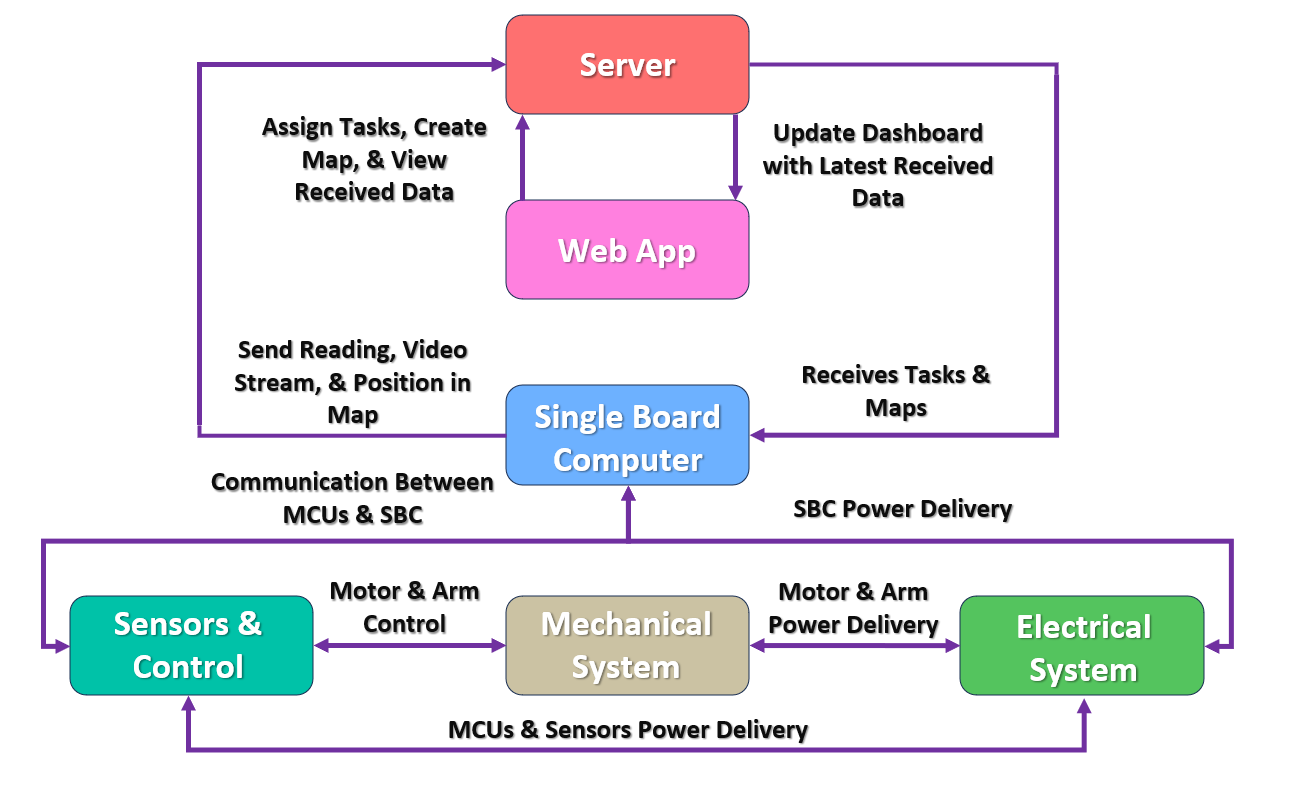
\includegraphics[scale=0.3]{./Figures/Intro/Capture.PNG}
	\caption{Block Diagram That Depicts System Architecture}
	\label{fig:sysarch}
\end{figure}

\section{What To Expect}
The next parts will include both the thought process behind each block implementation, used tools, as well as the expected outcome. The was the project is divided into section follows the depiction in the figure below.

\begin{figure}[h!]
	\centering
	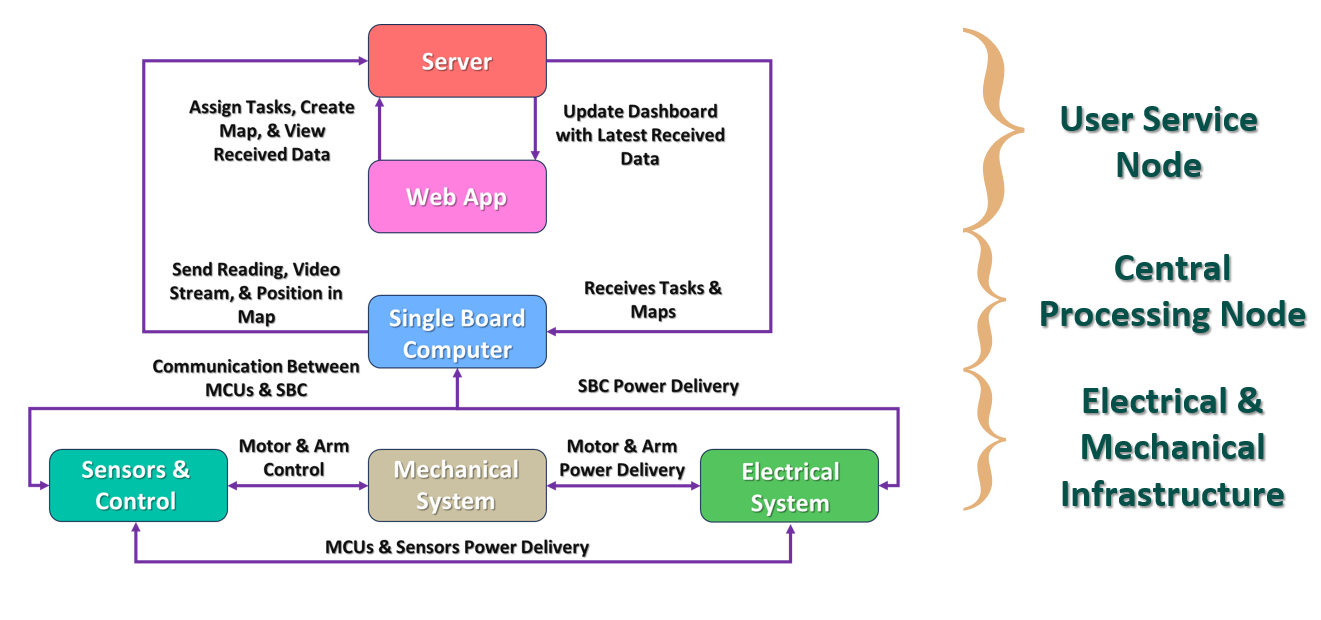
\includegraphics[scale=0.3]{./Figures/Intro/Capture2.PNG}
	\caption{Block Diagram That Depicts System Architecture (2)}
	\label{fig:sysarch}
\end{figure} 


